%%
%% This is file `sample-authordraft.tex',
%% generated with the docstrip utility.
%%
%% The original source files were:
%%
%% samples.dtx  (with options: `authordraft') changed it to review
%% 
%% IMPORTANT NOTICE:
%% 
%% For the copyright see the source file.
%% 
%% Any modified versions of this file must be renamed
%% with new filenames distinct from sample-authordraft.tex.
%% 
%% For distribution of the original source see the terms
%% for copying and modification in the file samples.dtx.
%% 
%% This generated file may be distributed as long as the
%% original source files, as listed above, are part of the
%% same distribution. (The sources need not necessarily be
%% in the same archive or directory.)
%%
%% The first command in your LaTeX source must be the \documentclass command.
\documentclass[sigconf,review]{acmart}

%%
%% \BibTeX command to typeset BibTeX logo in the docs
\AtBeginDocument{%
  \providecommand\BibTeX{{%
    \normalfont B\kern-0.5em{\scshape i\kern-0.25em b}\kern-0.8em\TeX}}}

\usepackage{graphicx}
\usepackage{multirow}
\usepackage{color, colortbl}
\usepackage{caption}
\usepackage{subcaption}
\usepackage{longtable}


%% Rights management information.  This information is sent to you
%% when you complete the rights form.  These commands have SAMPLE
%% values in them; it is your responsibility as an author to replace
%% the commands and values with those provided to you when you
%% complete the rights form.
\setcopyright{acmcopyright}
\copyrightyear{2019}
\acmYear{2019}
% FAHID UNCOMMENT \acmDOI{10.1145/1122445.1122456}

%% These commands are for a PROCEEDINGS abstract or paper.
% FAHID UNCOMMENT BLOCK
% \acmConference[Woodstock '18]{Woodstock '18: ACM Symposium on Neural
%   Gaze Detection}{June 03--05, 2018}{Woodstock, NY}
% \acmBooktitle{Woodstock '18: ACM Symposium on Neural Gaze Detection,
%   June 03--05, 2018, Woodstock, NY}
% \acmPrice{15.00}
% \acmISBN{978-1-4503-9999-9/18/06}


%%
%% Submission ID.
%% Use this when submitting an article to a sponsored event. You'll
%% receive a unique submission ID from the organizers
%% of the event, and this ID should be used as the parameter to this command.
%%\acmSubmissionID{123-A56-BU3}

%%
%% The majority of ACM publications use numbered citations and
%% references.  The command \citestyle{authoryear} switches to the
%% "author year" style.
%%
%% If you are preparing content for an event
%% sponsored by ACM SIGGRAPH, you must use the "author year" style of
%% citations and references.
%% Uncommenting
%% the next command will enable that style.
%%\citestyle{acmauthoryear}

%%
%% end of the preamble, start of the body of the document source.
\begin{document}

%%
%% The "title" command has an optional parameter,
%% allowing the author to define a "short title" to be used in page headers.
\title{TEMPORARY: CMU Study on Nichol's hypothesis}

%%
%% The "author" command and its associated commands are used to define
%% the authors and their affiliations.
%% Of note is the shared affiliation of the first two authors, and the
%% "authornote" and "authornotemark" commands
%% used to denote shared contribution to the research.
\author{Fahmid Morshed Fahid}
\authornote{All the authors contributed equally to this research.}
\email{ffahid@ncsu.edu}
\orcid{0000-0002-4802-3979}
\affiliation{%
  \institution{North Carolina State Univeristy}
  \streetaddress{Department of Computer Science}
  \city{Raleigh}
  \state{North Carolina}
  \postcode{27606}
}

\author{Tim Menzies}
\authornotemark[1]
\email{timm@ieee.org}
\orcid{0000-0002-5040-3196}
\affiliation{%
  \institution{North Carolina State Univeristy}
  \streetaddress{Department of Computer Science}
  \city{Raleigh}
  \state{North Carolina}
  \postcode{27606}
}

\author{William Nichols}
\authornotemark[1]
\email{wrn@sei.cmu.edu}
\orcid{0000-0002-1668-6882}
\affiliation{%
  \institution{Carnegie Mellon University Software Engineering Institute}
  \streetaddress{4500 Fifth Ave}
  \city{Pittsburgh}
  \state{Pennsylvania}
  \postcode{15213-2612}
}

%%
%% By default, the full list of authors will be used in the page
%% headers. Often, this list is too long, and will overlap
%% other information printed in the page headers. This command allows
%% the author to define a more concise list
%% of authors' names for this purpose.
\renewcommand{\shortauthors}{Fahmid et al.}
\newcommand{\quart}[4]{\begin{picture}(150,1)%1
{\color{black}\put(\numexpr #3 * 6  \relax,3){\circle*{4}}\put(\numexpr #1*6 \relax ,3){\line(1,0){\numexpr #2*6 \relax}}}\end{picture}}

\setlength{\tabcolsep}{2pt}
%%
%% The abstract is a short summary of the work to be presented in the
%% article.
\begin{abstract}
  A clear and well-documented \LaTeX\ document is presented as an
  article formatted for publication by ACM in a conference proceedings
  or journal publication. Based on the ``acmart'' document class, this
  article presents and explains many of the common variations, as well
  as many of the formatting elements an author may use in the
  preparation of the documentation of their work.
\end{abstract}

%%
%% The code below is generated by the tool at http://dl.acm.org/ccs.cfm.
%% Please copy and paste the code instead of the example below.
%%
\begin{CCSXML}
<ccs2012>
 <concept>
  <concept_id>10010520.10010553.10010562</concept_id>
  <concept_desc>Computer systems organization~Embedded systems</concept_desc>
  <concept_significance>500</concept_significance>
 </concept>
 <concept>
  <concept_id>10010520.10010575.10010755</concept_id>
  <concept_desc>Computer systems organization~Redundancy</concept_desc>
  <concept_significance>300</concept_significance>
 </concept>
 <concept>
  <concept_id>10010520.10010553.10010554</concept_id>
  <concept_desc>Computer systems organization~Robotics</concept_desc>
  <concept_significance>100</concept_significance>
 </concept>
 <concept>
  <concept_id>10003033.10003083.10003095</concept_id>
  <concept_desc>Networks~Network reliability</concept_desc>
  <concept_significance>100</concept_significance>
 </concept>
</ccs2012>
\end{CCSXML}

\ccsdesc[500]{Computer systems organization~Embedded systems}
\ccsdesc[300]{Computer systems organization~Redundancy}
\ccsdesc{Computer systems organization~Robotics}
\ccsdesc[100]{Networks~Network reliability}

%%
%% Keywords. The author(s) should pick words that accurately describe
%% the work being presented. Separate the keywords with commas.
\keywords{datasets, neural networks, gaze detection, text tagging}

%% A "teaser" image appears between the author and affiliation
%% information and the body of the document, and typically spans the
%% page.
\begin{teaserfigure}
  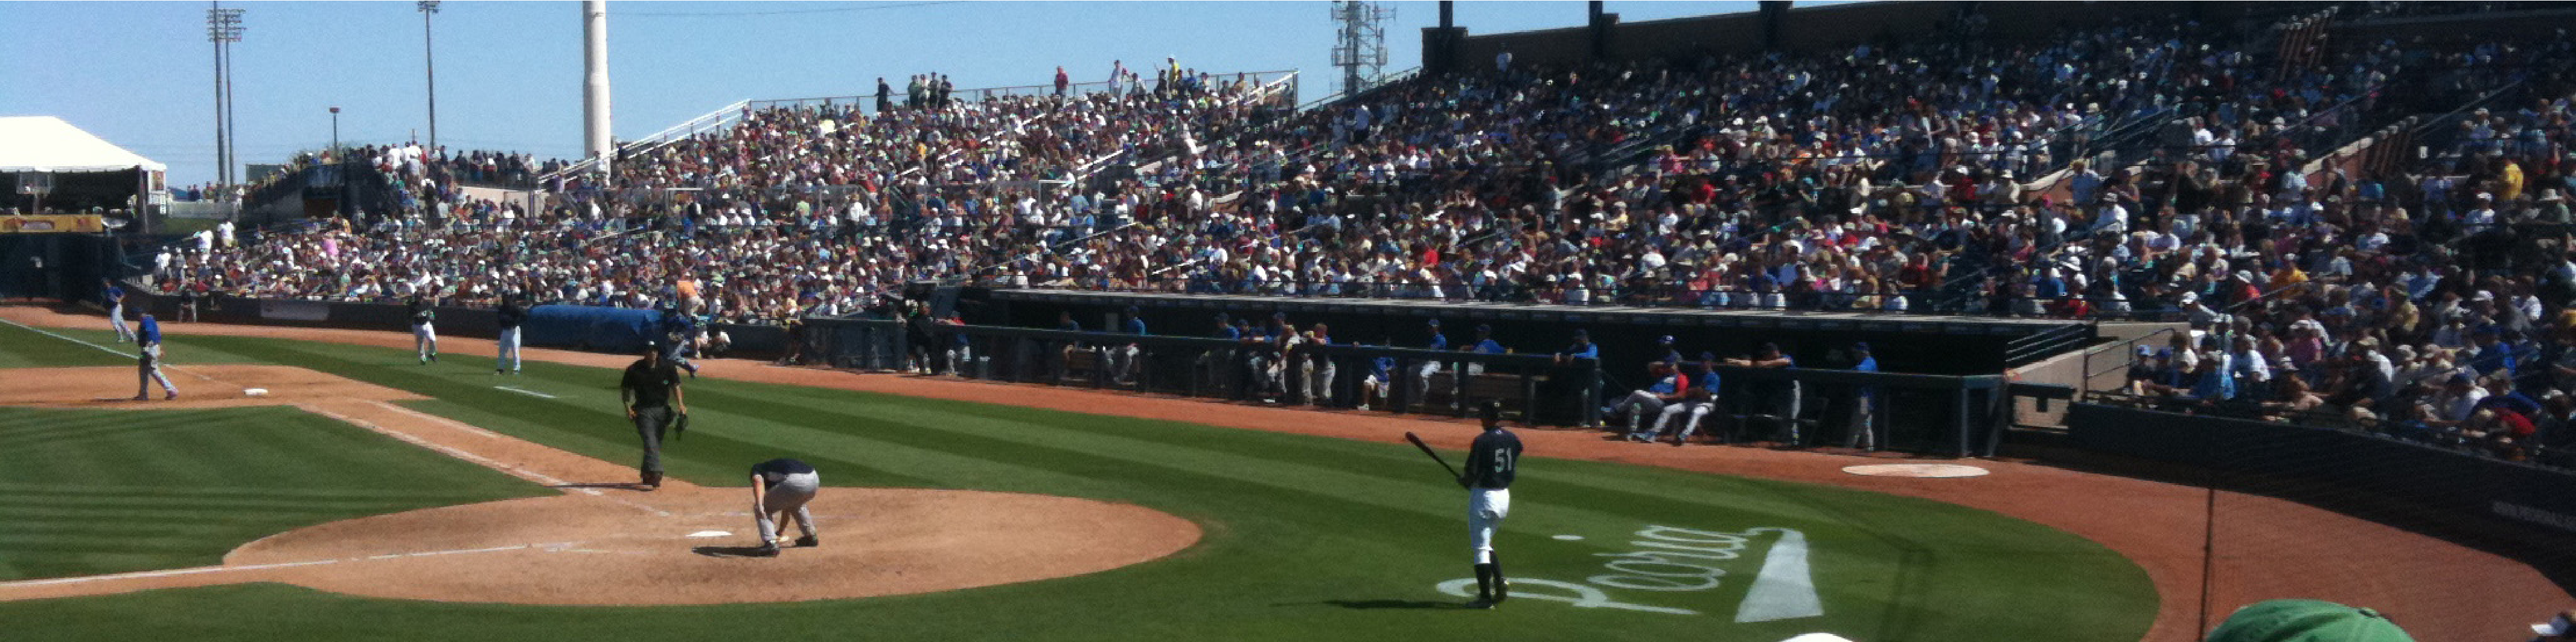
\includegraphics[width=\textwidth]{sampleteaser}
  \caption{Seattle Mariners at Spring Training, 2010.}
  \Description{Enjoying the baseball game from the third-base
  seats. Ichiro Suzuki preparing to bat.}
  \label{fig:teaser}
\end{teaserfigure}

%%
%% This command processes the author and affiliation and title
%% information and builds the first part of the formatted document.
\maketitle
\pagestyle{plain}
\section{Introduction}

\begin{table}
\centering
\caption{Overview of the Dataset}
\label{tab:overview}
\begin{tabular}{|l|l|l|l|l|}
\hline
\textbf{}       & \textbf{Size} & \textbf{Effort} & \textbf{Prod\_Rate} & \textbf{Defects} \\ \hline
\textbf{count}  & 16190       & 16190         & 16190             & 16190          \\ \hline
\textbf{median} & 96          & 197           & 48                & 6              \\ \hline
\textbf{iqr}    & 97          & 172           & 40                & 6             \\ \hline
\end{tabular}
\end{table}

% H0
\begin{table}

\scriptsize
\renewcommand{\baselinestretch}{.5} 
\centering
\caption{H0: Task overview with Size, Effort, Production Rate and Defects}
\label{tab:h0}
 \resizebox{\linewidth}{!}{
\begin{tabular}{|c|c|c|c|c|c|c|c|c|c|c|c|c|c|}
\hline
\textbf{} & \textbf{} & \multicolumn{3}{c|}{\textbf{size}} & \multicolumn{3}{c|}{\textbf{effort}} & \multicolumn{3}{c|}{\textbf{prod\_rate}} & \multicolumn{3}{c|}{\textbf{defect}} \\ \hline
\textbf{Task} & \textbf{\#} & \textbf{rank} & \textbf{med} & \textbf{iqr} & \textbf{rank} & \textbf{med} & \textbf{iqr} & \textbf{rank} & \textbf{med} & \textbf{iqr} & \textbf{rank} & \textbf{med} & \textbf{iqr} \\ \hline
\textbf{1} & \textbf{1619} & 2 & 81 & 90 & \cellcolor[HTML]{C0C0C0}1 & 146 & 132 & \cellcolor[HTML]{C0C0C0}1 & 56 & 54 & 3 & 7 & 7 \\ \hline
\textbf{2} & \textbf{1619} & \cellcolor[HTML]{C0C0C0}1 & 62 & 60 & \cellcolor[HTML]{C0C0C0}1 & 146 & 107 & 2 & 43 & 38 & 2 & 5 & 5 \\ \hline
\textbf{3} & \textbf{1619} & 2 & 72 & 78 & 2 & 183 & 149 & 2 & 41 & 39 & 3 & 6 & 6 \\ \hline
\textbf{4} & \textbf{1619} & 2 & 72 & 54 & \cellcolor[HTML]{C0C0C0}1 & 154 & 107 & 2 & 48 & 38 & \cellcolor[HTML]{C0C0C0}1 & 4 & 5 \\ \hline
\textbf{5} & \textbf{1619} & 2 & 81 & 54 & 2 & 168 & 124 & 2 & 48 & 37 & 2 & 5 & 5 \\ \hline
\textbf{6} & \textbf{1619} & 3 & 153 & 93 & 3 & 288 & 234 & 2 & 51 & 41 & 3 & 7 & 8 \\ \hline
\textbf{7} & \textbf{1619} & 2 & 81 & 60 & 2 & 202 & 134 & 2 & 40 & 34 & 2 & 5 & 4 \\ \hline
\textbf{8} & \textbf{1619} & 2 & 75 & 59 & \cellcolor[HTML]{C0C0C0}1 & 163 & 142 & 2 & 44 & 36 & \cellcolor[HTML]{C0C0C0}1 & 4 & 5 \\ \hline
\textbf{9} & \textbf{1619} & 3 & 142 & 102 & 3 & 284 & 209 & 2 & 50 & 36 & 3 & 7 & 7 \\ \hline
\textbf{10} & \textbf{1619} & 4 & 208 & 120 & 4 & 334 & 253 & \cellcolor[HTML]{C0C0C0}1 & 60 & 41 & 3 & 7 & 7 \\ \hline
\end{tabular}
}
\end{table}



% Scope 1

% H1a
\begin{table}
\scriptsize
\renewcommand{\baselinestretch}{0.5} 
\centering
\caption{H1a: Productivity varies across different language categories and same within the category
}
\label{tab:h1a}
\begin{tabular}{|c|c|c|c|c|}
\hline
\textbf{Task} & \textbf{Category} & \textbf{count} & \textbf{size} & \textbf{effort} \\ \hline
 & \textbf{OO} & 771 & 99 & 154 \\ \cline{2-5} 
 & \textbf{PO} & 725 & 74 & 149 \\ \cline{2-5} 
 & \textbf{SL} & 15 & \cellcolor[HTML]{C0C0C0}59 & 142 \\ \cline{2-5} 
\multirow{-4}{*}{\textbf{1}} & \textbf{VD} & 63 & \cellcolor[HTML]{C0C0C0}40 & \cellcolor[HTML]{C0C0C0}98 \\ \hline
 & \textbf{OO} & 771 & 71 & 147 \\ \cline{2-5} 
 & \textbf{PO} & 725 & 56 & 149 \\ \cline{2-5} 
 & \textbf{SL} & 15 & \cellcolor[HTML]{C0C0C0}54 & 177 \\ \cline{2-5} 
\multirow{-4}{*}{\textbf{2}} & \textbf{VD} & 63 & \cellcolor[HTML]{C0C0C0}42 & \cellcolor[HTML]{C0C0C0}99 \\ \hline
 & \textbf{OO} & 771 & 93 & 199 \\ \cline{2-5} 
 & \textbf{PO} & 725 & \cellcolor[HTML]{C0C0C0}61 & 173 \\ \cline{2-5} 
 & \textbf{SL} & 15 & \cellcolor[HTML]{C0C0C0}57 & 223 \\ \cline{2-5} 
\multirow{-4}{*}{\textbf{3}} & \textbf{VD} & 63 & \cellcolor[HTML]{C0C0C0}55 & \cellcolor[HTML]{C0C0C0}148 \\ \hline
 & \textbf{OO} & 771 & 82 & \cellcolor[HTML]{C0C0C0}156 \\ \cline{2-5} 
 & \textbf{PO} & 725 & \cellcolor[HTML]{C0C0C0}66 & \cellcolor[HTML]{C0C0C0}149 \\ \cline{2-5} 
 & \textbf{SL} & 15 & \cellcolor[HTML]{C0C0C0}75 & \cellcolor[HTML]{C0C0C0}132 \\ \cline{2-5} 
\multirow{-4}{*}{\textbf{4}} & \textbf{VD} & 63 & \cellcolor[HTML]{C0C0C0}54 & \cellcolor[HTML]{C0C0C0}143 \\ \hline
 & \textbf{OO} & 771 & 91 & \cellcolor[HTML]{C0C0C0}168 \\ \cline{2-5} 
 & \textbf{PO} & 725 & 73 & \cellcolor[HTML]{C0C0C0}167 \\ \cline{2-5} 
 & \textbf{SL} & 15 & \cellcolor[HTML]{C0C0C0}62 & \cellcolor[HTML]{C0C0C0}215 \\ \cline{2-5} 
\multirow{-4}{*}{\textbf{5}} & \textbf{VD} & 63 & \cellcolor[HTML]{C0C0C0}64 & \cellcolor[HTML]{C0C0C0}170 \\ \hline
 & \textbf{OO} & 771 & 165 & \cellcolor[HTML]{C0C0C0}286 \\ \cline{2-5} 
 & \textbf{PO} & 725 & \cellcolor[HTML]{C0C0C0}145 & \cellcolor[HTML]{C0C0C0}293 \\ \cline{2-5} 
 & \textbf{SL} & 15 & \cellcolor[HTML]{C0C0C0}144 & \cellcolor[HTML]{C0C0C0}344 \\ \cline{2-5} 
\multirow{-4}{*}{\textbf{6}} & \textbf{VD} & 63 & \cellcolor[HTML]{C0C0C0}145 & \cellcolor[HTML]{C0C0C0}258 \\ \hline
 & \textbf{OO} & 771 & \cellcolor[HTML]{C0C0C0}85 & \cellcolor[HTML]{C0C0C0}201 \\ \cline{2-5} 
 & \textbf{PO} & 725 & \cellcolor[HTML]{C0C0C0}78 & \cellcolor[HTML]{C0C0C0}204 \\ \cline{2-5} 
 & \textbf{SL} & 15 & \cellcolor[HTML]{C0C0C0}83 & \cellcolor[HTML]{C0C0C0}218 \\ \cline{2-5} 
\multirow{-4}{*}{\textbf{7}} & \textbf{VD} & 63 & \cellcolor[HTML]{C0C0C0}88 & \cellcolor[HTML]{C0C0C0}192 \\ \hline
 & \textbf{OO} & 771 & 82 & \cellcolor[HTML]{C0C0C0}165 \\ \cline{2-5} 
 & \textbf{PO} & 725 & \cellcolor[HTML]{C0C0C0}71 & \cellcolor[HTML]{C0C0C0}162 \\ \cline{2-5} 
 & \textbf{SL} & 15 & \cellcolor[HTML]{C0C0C0}51 & \cellcolor[HTML]{C0C0C0}165 \\ \cline{2-5} 
\multirow{-4}{*}{\textbf{8}} & \textbf{VD} & 63 & \cellcolor[HTML]{C0C0C0}48 & \cellcolor[HTML]{C0C0C0}142 \\ \hline
 & \textbf{OO} & 771 & 156 & \cellcolor[HTML]{C0C0C0}289 \\ \cline{2-5} 
 & \textbf{PO} & 725 & \cellcolor[HTML]{C0C0C0}133 & \cellcolor[HTML]{C0C0C0}285 \\ \cline{2-5} 
 & \textbf{SL} & 15 & \cellcolor[HTML]{C0C0C0}117 & \cellcolor[HTML]{C0C0C0}274 \\ \cline{2-5} 
\multirow{-4}{*}{\textbf{9}} & \textbf{VD} & 63 & 156 & \cellcolor[HTML]{C0C0C0}250 \\ \hline
 & \textbf{OO} & 771 & 223 & \cellcolor[HTML]{C0C0C0}342 \\ \cline{2-5} 
 & \textbf{PO} & 725 & \cellcolor[HTML]{C0C0C0}193 & \cellcolor[HTML]{C0C0C0}328 \\ \cline{2-5} 
 & \textbf{SL} & 15 & \cellcolor[HTML]{C0C0C0}183 & \cellcolor[HTML]{C0C0C0}351 \\ \cline{2-5} 
\multirow{-4}{*}{\textbf{10}} & \textbf{VD} & 63 & 217 & \cellcolor[HTML]{C0C0C0}287 \\ \hline
\multicolumn{3}{|c|}{\textit{\textbf{TOP RANKED}}} & \textit{\textbf{\begin{tabular}[c]{@{}c@{}}OO=0, PO=7,\\ SL=10, VD=8\end{tabular}}} & \textit{\textbf{\begin{tabular}[c]{@{}c@{}}OO=7, PO=7,\\ SL=7, VD=10\end{tabular}}} \\ \hline
\end{tabular}
\end{table}



% H1b 4GL is twice as productive as 3GL

\begin{table}

\scriptsize
\renewcommand{\baselinestretch}{0.5} 

\centering
\caption{H1b: 4GL is twice as productive as 3GL}
\label{tab:h1b}
\begin{tabular}{|c|c|c|c|c|}
\hline
\textbf{Task} & \textbf{PL\_Gen} & \textbf{count} & \textbf{size} & \textbf{effort} \\ \hline
 & \textbf{3} & 1451 & 86 & 151 \\ \cline{2-5} 
\multirow{-2}{*}{\textbf{1}} & \textbf{4} & 103 & \cellcolor[HTML]{C0C0C0}45 & \cellcolor[HTML]{C0C0C0}105 \\ \hline
 & \textbf{3} & 1451 & 63 & 147 \\ \cline{2-5} 
\multirow{-2}{*}{\textbf{2}} & \textbf{4} & 103 & \cellcolor[HTML]{C0C0C0}43 & \cellcolor[HTML]{C0C0C0}110 \\ \hline
 & \textbf{3} & 1451 & 74 & 185 \\ \cline{2-5} 
\multirow{-2}{*}{\textbf{3}} & \textbf{4} & 103 & \cellcolor[HTML]{C0C0C0}57 & \cellcolor[HTML]{C0C0C0}152 \\ \hline
 & \textbf{3} & 1451 & 74 & \cellcolor[HTML]{C0C0C0}154 \\ \cline{2-5} 
\multirow{-2}{*}{\textbf{4}} & \textbf{4} & 103 & \cellcolor[HTML]{C0C0C0}54 & \cellcolor[HTML]{C0C0C0}139 \\ \hline
 & \textbf{3} & 1451 & 82 & \cellcolor[HTML]{C0C0C0}168 \\ \cline{2-5} 
\multirow{-2}{*}{\textbf{5}} & \textbf{4} & 103 & \cellcolor[HTML]{C0C0C0}55 & \cellcolor[HTML]{C0C0C0}158 \\ \hline
 & \textbf{3} & 1451 & 155 & 292 \\ \cline{2-5} 
\multirow{-2}{*}{\textbf{6}} & \textbf{4} & 103 & \cellcolor[HTML]{C0C0C0}128 & \cellcolor[HTML]{C0C0C0}225 \\ \hline
 & \textbf{3} & 1451 & \cellcolor[HTML]{C0C0C0}82 & \cellcolor[HTML]{C0C0C0}202 \\ \cline{2-5} 
\multirow{-2}{*}{\textbf{7}} & \textbf{4} & 103 & \cellcolor[HTML]{C0C0C0}80 & \cellcolor[HTML]{C0C0C0}190 \\ \hline
 & \textbf{3} & 1451 & 77 & \cellcolor[HTML]{C0C0C0}163 \\ \cline{2-5} 
\multirow{-2}{*}{\textbf{8}} & \textbf{4} & 103 & \cellcolor[HTML]{C0C0C0}51 & \cellcolor[HTML]{C0C0C0}148 \\ \hline
 & \textbf{3} & 1451 & 142 & 288 \\ \cline{2-5} 
\multirow{-2}{*}{\textbf{9}} & \textbf{4} & 103 & \cellcolor[HTML]{C0C0C0}120 & \cellcolor[HTML]{C0C0C0}227 \\ \hline
 & \textbf{3} & 1451 & 209 & 336 \\ \cline{2-5} 
\multirow{-2}{*}{\textbf{10}} & \textbf{4} & 103 & \cellcolor[HTML]{C0C0C0}185 & \cellcolor[HTML]{C0C0C0}284 \\ \hline
\multicolumn{3}{|c|}{\textit{\textbf{TOP RANKED}}} & \textit{\textbf{3G=1, 4G=10}} & \textit{\textbf{3G=4, 4G=10}} \\ \hline
\end{tabular}
\end{table}

% H1c Average number of LOC is proportional to PL Level

\begin{table}
\scriptsize
\renewcommand{\baselinestretch}{0.5} 
\centering
\caption{H1c: Average number of LOC is proportional to PL Level}
\label{tab:h1c}
\resizebox{\linewidth}{!}{
\begin{tabular}{|c@{~}|c@{~}|c@{~}|c@{~}|c@{~}|c@{~}|c@{~}|c@{~}|c|}
\hline
\textbf{} & \textbf{} & \textbf{} & \multicolumn{3}{c|}{\textbf{size}} & \multicolumn{3}{c|}{\textbf{effort}} \\ \hline
\textbf{Task} & \textbf{Level\_Bin} & \textbf{count} & \textbf{rank} & \textbf{median} & \textbf{iqr} & \textbf{rank} & \textbf{median} & \textbf{iqr} \\ \hline
 & \textbf{1-4} & 728 & \cellcolor[HTML]{EFEFEF}2 & 82 & 89 & 3 & 165 & 144 \\ \cline{2-9} 
 & \textbf{5-8} & 364 & 3 & 105 & 117 & 3 & 181 & 132 \\ \cline{2-9} 
 & \textbf{9-12} & 216 & \cellcolor[HTML]{EFEFEF}2 & 69 & 84 & \cellcolor[HTML]{EFEFEF}2 & 128 & 98 \\ \cline{2-9} 
 & \textbf{13-16} & 17 & \cellcolor[HTML]{C0C0C0}1 & 0 & 64 & 3 & 168 & 157 \\ \cline{2-9} 
 & \textbf{17-20} & 33 & \cellcolor[HTML]{C0C0C0}1 & 52 & 45 & \cellcolor[HTML]{EFEFEF}2 & 132 & 76 \\ \cline{2-9} 
\multirow{-6}{*}{\textbf{1}} & \textbf{25-28} & 28 & \cellcolor[HTML]{C0C0C0}1 & 46 & 35 & \cellcolor[HTML]{C0C0C0}1 & 85 & 47 \\ \hline
 & \textbf{1-4} & 728 & \cellcolor[HTML]{EFEFEF}2 & 60 & 53 & 3 & 160 & 113 \\ \cline{2-9} 
 & \textbf{5-8} & 364 & 3 & 72 & 68 & 3 & 167 & 103 \\ \cline{2-9} 
 & \textbf{9-12} & 216 & \cellcolor[HTML]{EFEFEF}2 & 56 & 68 & \cellcolor[HTML]{EFEFEF}2 & 130 & 99 \\ \cline{2-9} 
 & \textbf{13-16} & 17 & \cellcolor[HTML]{C0C0C0}1 & 41 & 33 & 3 & 158 & 105 \\ \cline{2-9} 
 & \textbf{17-20} & 33 & \cellcolor[HTML]{C0C0C0}1 & 37 & 44 & \cellcolor[HTML]{EFEFEF}2 & 130 & 81 \\ \cline{2-9} 
\multirow{-6}{*}{\textbf{2}} & \textbf{25-28} & 28 & \cellcolor[HTML]{C0C0C0}1 & 32 & 45 & \cellcolor[HTML]{C0C0C0}1 & 78 & 44 \\ \hline
 & \textbf{1-4} & 728 & 3 & 65 & 61 & \cellcolor[HTML]{EFEFEF}2 & 182 & 156 \\ \cline{2-9} 
 & \textbf{5-8} & 364 & 4 & 108 & 124 & 3 & 242 & 190 \\ \cline{2-9} 
 & \textbf{9-12} & 216 & 3 & 67 & 67 & \cellcolor[HTML]{EFEFEF}2 & 168 & 110 \\ \cline{2-9} 
 & \textbf{13-16} & 17 & \cellcolor[HTML]{C0C0C0}1 & 34 & 34 & \cellcolor[HTML]{EFEFEF}2 & 205 & 100 \\ \cline{2-9} 
 & \textbf{17-20} & 33 & \cellcolor[HTML]{EFEFEF}2 & 57 & 67 & \cellcolor[HTML]{EFEFEF}2 & 150 & 96 \\ \cline{2-9} 
\multirow{-6}{*}{\textbf{3}} & \textbf{25-28} & 28 & \cellcolor[HTML]{EFEFEF}2 & 54 & 59 & \cellcolor[HTML]{C0C0C0}1 & 129 & 65 \\ \hline
 & \textbf{1-4} & 728 & \cellcolor[HTML]{EFEFEF}2 & 69 & 46 & 3 & 155 & 119 \\ \cline{2-9} 
 & \textbf{5-8} & 364 & 3 & 81 & 61 & 3 & 162 & 124 \\ \cline{2-9} 
 & \textbf{9-12} & 216 & \cellcolor[HTML]{EFEFEF}2 & 71 & 60 & 3 & 167 & 91 \\ \cline{2-9} 
 & \textbf{13-16} & 17 & \cellcolor[HTML]{EFEFEF}2 & 73 & 49 & 4 & 300 & 379 \\ \cline{2-9} 
 & \textbf{17-20} & 33 & \cellcolor[HTML]{C0C0C0}1 & 51 & 38 & \cellcolor[HTML]{EFEFEF}2 & 149 & 63 \\ \cline{2-9} 
\multirow{-6}{*}{\textbf{4}} & \textbf{25-28} & 28 & \cellcolor[HTML]{C0C0C0}1 & 51 & 37 & \cellcolor[HTML]{C0C0C0}1 & 99 & 49 \\ \hline
 & \textbf{1-4} & 728 & \cellcolor[HTML]{EFEFEF}2 & 78 & 49 & \cellcolor[HTML]{EFEFEF}2 & 173 & 125 \\ \cline{2-9} 
 & \textbf{5-8} & 364 & 3 & 91 & 64 & \cellcolor[HTML]{EFEFEF}2 & 181 & 134 \\ \cline{2-9} 
 & \textbf{9-12} & 216 & \cellcolor[HTML]{EFEFEF}2 & 70 & 50 & \cellcolor[HTML]{EFEFEF}2 & 178 & 128 \\ \cline{2-9} 
 & \textbf{13-16} & 17 & \cellcolor[HTML]{EFEFEF}2 & 67 & 92 & 3 & 275 & 198 \\ \cline{2-9} 
 & \textbf{17-20} & 33 & \cellcolor[HTML]{C0C0C0}1 & 50 & 20 & \cellcolor[HTML]{C0C0C0}1 & 120 & 86 \\ \cline{2-9} 
\multirow{-6}{*}{\textbf{5}} & \textbf{25-28} & 28 & 3 & 87 & 36 & \cellcolor[HTML]{C0C0C0}1 & 132 & 76 \\ \hline
 & \textbf{1-4} & 728 & \cellcolor[HTML]{EFEFEF}2 & 151 & 81 & \cellcolor[HTML]{EFEFEF}2 & 315 & 237 \\ \cline{2-9} 
 & \textbf{5-8} & 364 & 3 & 172 & 102 & \cellcolor[HTML]{EFEFEF}2 & 302 & 245 \\ \cline{2-9} 
 & \textbf{9-12} & 216 & \cellcolor[HTML]{EFEFEF}2 & 145 & 89 & \cellcolor[HTML]{EFEFEF}2 & 268 & 222 \\ \cline{2-9} 
 & \textbf{13-16} & 17 & \cellcolor[HTML]{EFEFEF}2 & 135 & 108 & \cellcolor[HTML]{EFEFEF}2 & 416 & 251 \\ \cline{2-9} 
 & \textbf{17-20} & 33 & \cellcolor[HTML]{C0C0C0}1 & 85 & 90 & \cellcolor[HTML]{C0C0C0}1 & 179 & 136 \\ \cline{2-9} 
\multirow{-6}{*}{\textbf{6}} & \textbf{25-28} & 28 & \cellcolor[HTML]{EFEFEF}2 & 159 & 146 & \cellcolor[HTML]{C0C0C0}1 & 178 & 164 \\ \hline
 & \textbf{1-4} & 728 & \cellcolor[HTML]{EFEFEF}2 & 80 & 59 & \cellcolor[HTML]{C0C0C0}1 & 212 & 146 \\ \cline{2-9} 
 & \textbf{5-8} & 364 & \cellcolor[HTML]{EFEFEF}2 & 83 & 63 & \cellcolor[HTML]{C0C0C0}1 & 213 & 123 \\ \cline{2-9} 
 & \textbf{9-12} & 216 & \cellcolor[HTML]{EFEFEF}2 & 82 & 68 & \cellcolor[HTML]{C0C0C0}1 & 212 & 122 \\ \cline{2-9} 
 & \textbf{13-16} & 17 & \cellcolor[HTML]{EFEFEF}2 & 88 & 44 & \cellcolor[HTML]{C0C0C0}1 & 308 & 209 \\ \cline{2-9} 
 & \textbf{17-20} & 33 & \cellcolor[HTML]{C0C0C0}1 & 62 & 52 & \cellcolor[HTML]{C0C0C0}1 & 163 & 91 \\ \cline{2-9} 
\multirow{-6}{*}{\textbf{7}} & \textbf{25-28} & 28 & \cellcolor[HTML]{EFEFEF}2 & 86 & 65 & \cellcolor[HTML]{C0C0C0}1 & 157 & 92 \\ \hline
 & \textbf{1-4} & 728 & \cellcolor[HTML]{EFEFEF}2 & 75 & 59 & 3 & 176 & 174 \\ \cline{2-9} 
 & \textbf{5-8} & 364 & 3 & 85 & 65 & 3 & 189 & 137 \\ \cline{2-9} 
 & \textbf{9-12} & 216 & \cellcolor[HTML]{EFEFEF}2 & 73 & 50 & 3 & 165 & 113 \\ \cline{2-9} 
 & \textbf{13-16} & 17 & \cellcolor[HTML]{C0C0C0}1 & 61 & 44 & 4 & 316 & 78 \\ \cline{2-9} 
 & \textbf{17-20} & 33 & \cellcolor[HTML]{C0C0C0}1 & 54 & 42 & \cellcolor[HTML]{EFEFEF}2 & 140 & 78 \\ \cline{2-9} 
\multirow{-6}{*}{\textbf{8}} & \textbf{25-28} & 28 & \cellcolor[HTML]{C0C0C0}1 & 42 & 40 & \cellcolor[HTML]{C0C0C0}1 & 81 & 50 \\ \hline
 & \textbf{1-4} & 728 & \cellcolor[HTML]{C0C0C0}1 & 137 & 89 & \cellcolor[HTML]{EFEFEF}2 & 300 & 218 \\ \cline{2-9} 
 & \textbf{5-8} & 364 & \cellcolor[HTML]{C0C0C0}1 & 162 & 120 & \cellcolor[HTML]{EFEFEF}2 & 311 & 237 \\ \cline{2-9} 
 & \textbf{9-12} & 216 & \cellcolor[HTML]{C0C0C0}1 & 144 & 96 & \cellcolor[HTML]{EFEFEF}2 & 282 & 191 \\ \cline{2-9} 
 & \textbf{13-16} & 17 & \cellcolor[HTML]{C0C0C0}1 & 122 & 91 & \cellcolor[HTML]{EFEFEF}2 & 445 & 130 \\ \cline{2-9} 
 & \textbf{17-20} & 33 & \cellcolor[HTML]{C0C0C0}1 & 88 & 73 & \cellcolor[HTML]{C0C0C0}1 & 179 & 89 \\ \cline{2-9} 
\multirow{-6}{*}{\textbf{9}} & \textbf{25-28} & 28 & \cellcolor[HTML]{C0C0C0}1 & 154 & 118 & \cellcolor[HTML]{C0C0C0}1 & 214 & 150 \\ \hline
 & \textbf{1-4} & 728 & \cellcolor[HTML]{EFEFEF}2 & 200 & 115 & \cellcolor[HTML]{EFEFEF}2 & 352 & 275 \\ \cline{2-9} 
 & \textbf{5-8} & 364 & 3 & 227 & 119 & \cellcolor[HTML]{EFEFEF}2 & 382 & 283 \\ \cline{2-9} 
 & \textbf{9-12} & 216 & \cellcolor[HTML]{EFEFEF}2 & 200 & 123 & \cellcolor[HTML]{C0C0C0}1 & 312 & 208 \\ \cline{2-9} 
 & \textbf{13-16} & 17 & 3 & 253 & 145 & 3 & 702 & 333 \\ \cline{2-9} 
 & \textbf{17-20} & 33 & \cellcolor[HTML]{C0C0C0}1 & 144 & 114 & \cellcolor[HTML]{C0C0C0}1 & 260 & 121 \\ \cline{2-9} 
\multirow{-6}{*}{\textbf{10}} & \textbf{25-28} & 28 & 3 & 220 & 148 & \cellcolor[HTML]{C0C0C0}1 & 256 & 175 \\ \hline
\multicolumn{3}{|c|}{\textit{\textbf{TOP RANKED}}} & \multicolumn{3}{c|}{\textit{\textbf{\begin{tabular}[c]{@{}c@{}}1-4=1, 4-8=1, 9-12=1,\\ 13-16=5, 17-20=9, 25-28=5\end{tabular}}}} & \multicolumn{3}{c|}{\textit{\textbf{\begin{tabular}[c]{@{}c@{}}1-4=1, 4-8=1, 9-12=2,\\ 13-16=1, 17-20=5, 25-28=10\end{tabular}}}} \\ \hline
\end{tabular}
}
\end{table}


\begin{figure}[!t]
\begin{center}
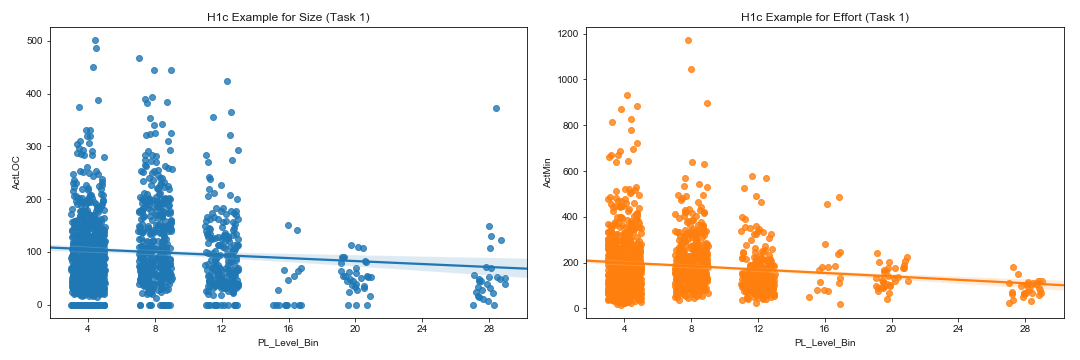
\includegraphics[width=\linewidth]{resources/h1c_example.png}
\caption{H1c example plot for task 1: Average number of LOC is proportional to PL Level}
\label{fig:h1c_example}
\end{center}
\end{figure}

% H1d
NOTE: We tried to produce H1d: Perl Python Rexx Tcl (D1) takes half time than C C++ Java (D2). But we only had 16 examples on D1 and 1200 examples of D2, which we though is very biased. Though our disagree with the claim (they are mostly equivalent), but due to biased data, we can not make any comment on this. 

% Scope 2
% h2 PL do not affect productivity
\begin{figure}[!t]
 
\centering
{\scriptsize
\renewcommand{\baselinestretch}{.5} 
{ \begin{tabular}{l@{~~~}l@{~~~}r@{~~~}r@{~~~}c}
\arrayrulecolor{darkgray}
\rowcolor[gray]{.9}  rank & PL & median & IQR & \\
    1 &      IDF &    2 &  2 & \quart{1}{2}{2}{100} \\
    1 &      MUMPS &    3 &  2 & \quart{2}{2}{3}{100} \\
    2 &      BAAN4GL &    5 &  3 & \quart{5}{3}{5}{100} \\
    2 &      SAS &    5 &  5 & \quart{3}{5}{5}{100} \\
    2 &      P &    5 &  6 & \quart{3}{6}{5}{100} \\
    2 &      ASP.NET &    5 &  3 & \quart{3}{3}{5}{100} \\
    2 &      X &    6 &  5 & \quart{4}{5}{6}{100} \\
    2 &      SMALLTALK &    6 &  8 & \quart{3}{8}{6}{100} \\
    3 &      JAVASCRIPT &    6 &  5 & \quart{5}{5}{6}{100} \\
    3 &      TSQL &    7 &  5 & \quart{5}{5}{7}{100} \\
    3 &      VAXFORTRAN &    6 &  7 & \quart{5}{7}{6}{100} \\
    3 &      NATURAL &    7 &  3 & \quart{6}{3}{7}{100} \\
    3 &      POWERBUILDER &    7 &  5 & \quart{5}{5}{7}{100} \\
    3 &      SQL &    7 &  9 & \quart{4}{9}{7}{100} \\
    3 &      PROGRESS &    7 &  9 & \quart{4}{9}{7}{100} \\
    3 &      UNIFASE &    7 &  6 & \quart{4}{6}{7}{100} \\
    3 &      PHP &    7 &  3 & \quart{6}{3}{7}{100} \\
    3 &      X++ &    8 &  5 & \quart{6}{5}{8}{100} \\
    3 &      PERL &    8 &  10 & \quart{4}{10}{8}{100} \\
    3 &      C &    8 &  8 & \quart{5}{8}{8}{100} \\
    3 &      FORTRAN &    8 &  4 & \quart{8}{4}{8}{100} \\
    3 &      ADA &    8 &  10 & \quart{5}{10}{8}{100} \\
    3 &      COBOL &    8 &  10 & \quart{4}{10}{8}{100} \\
    3 &      VB &    9 &  9 & \quart{5}{9}{9}{100} \\
    3 &      RPG &    8 &  12 & \quart{5}{12}{8}{100} \\
    3 &      F &    9 &  7 & \quart{6}{7}{9}{100} \\
    3 &      C\# &    9 &  9 & \quart{6}{9}{9}{100} \\
    4 &      PASCAL &    10 &  7 & \quart{7}{7}{10}{100} \\
    4 &      J &    10 &  13 & \quart{8}{13}{10}{100} \\
    4 &      4JS &    9 &  6 & \quart{6}{6}{9}{100} \\
    4 &      JAVA &    10 &  10 & \quart{6}{10}{10}{100} \\
    4 &      LOTUS\_SCRIPT &    10 &  9 & \quart{6}{9}{10}{100} \\
    4 &      MFC &    9 &  8 & \quart{6}{8}{9}{100} \\
    4 &      DELPHI &    11 &  6 & \quart{9}{6}{11}{100} \\
    4 &      C++ &    11 &  10 & \quart{7}{10}{11}{100} \\
    4 &      JOVIAL &    11 &  13 & \quart{6}{13}{11}{100} \\
    4 &      VC++ &    12 &  11 & \quart{8}{11}{12}{100} \\
    4 &      COLDFUSION &    13 &  7 & \quart{12}{7}{13}{100} \\
\end{tabular}}
}
\caption{H2 Size: PL do not affect productivity
}\label{fig:h2 size}
\end{figure}



\begin{figure}[!t]
\centering

{\scriptsize
\renewcommand{\baselinestretch}{.5} 
{  \begin{tabular}{l@{~~~}l@{~~~}r@{~~~}r@{~~~}c}
\arrayrulecolor{darkgray}
\rowcolor[gray]{.9}  rank & PL & median & IQR & \\
    1 &      MFC &    2 &  2 & \quart{1}{2}{2}{100} \\
    1 &      MUMPS &    2 &  1 & \quart{2}{1}{2}{100} \\
    1 &      TSQL &    3 &  2 & \quart{2}{2}{3}{100} \\
    1 &      RPG &    3 &  3 & \quart{2}{3}{3}{100} \\
    1 &      NATURAL &    3 &  3 & \quart{2}{3}{3}{100} \\
    1 &      ASP.NET &    3 &  1 & \quart{2}{1}{3}{100} \\
    1 &      P &    3 &  2 & \quart{2}{2}{3}{100} \\
    1 &      C\# &    3 &  3 & \quart{2}{3}{3}{100} \\
    1 &      SQL &    3 &  2 & \quart{2}{2}{3}{100} \\
    1 &      X++ &    3 &  4 & \quart{2}{4}{3}{100} \\
    1 &      LOTUS\_SCRIPT &    4 &  3 & \quart{3}{3}{4}{100} \\
    1 &      VB &    4 &  3 & \quart{3}{3}{4}{100} \\
    1 &      SAS &    4 &  3 & \quart{2}{3}{4}{100} \\
    1 &      C &    4 &  4 & \quart{3}{4}{4}{100} \\
    1 &      POWERBUILDER &    4 &  3 & \quart{2}{3}{4}{100} \\
    1 &      X &    4 &  2 & \quart{3}{2}{4}{100} \\
    1 &      DELPHI &    4 &  1 & \quart{4}{1}{4}{100} \\
    1 &      COBOL &    4 &  4 & \quart{2}{4}{4}{100} \\
    1 &      IDF &    4 &  2 & \quart{4}{2}{4}{100} \\
    1 &      PHP &    4 &  2 & \quart{4}{2}{4}{100} \\
    1 &      BAAN4GL &    5 &  3 & \quart{3}{3}{5}{100} \\
    1 &      C++ &    5 &  4 & \quart{3}{4}{5}{100} \\
    1 &      4JS &    5 &  3 & \quart{4}{3}{5}{100} \\
    1 &      PROGRESS &    5 &  4 & \quart{3}{4}{5}{100} \\
    1 &      cat\_JAVA &    5 &  4 & \quart{3}{4}{5}{100} \\
    1 &      FORTRAN &    5 &  3 & \quart{4}{3}{5}{100} \\
    1 &      PASCAL &    6 &  6 & \quart{4}{6}{6}{100} \\
    1 &      PERL &    6 &  8 & \quart{3}{8}{6}{100} \\
    1 &      UNIFASE &    6 &  3 & \quart{5}{3}{6}{100} \\
    1 &      J &    6 &  8 & \quart{5}{8}{6}{100} \\
    1 &      VC++ &    6 &  5 & \quart{4}{5}{6}{100} \\
    1 &      F &    7 &  5 & \quart{4}{5}{7}{100} \\
    1 &      SMALLTALK &    7 &  6 & \quart{4}{6}{7}{100} \\
    1 &      JAVASCRIPT &    7 &  4 & \quart{5}{4}{7}{100} \\
    1 &      COLDFUSION &    7 &  4 & \quart{5}{4}{7}{100} \\
    1 &      ADA &    8 &  7 & \quart{5}{7}{8}{100} \\
    2 &      VAXFORTRAN &    9 &  4 & \quart{8}{4}{9}{100} \\
    2 &      JOVIAL &    11 &  11 & \quart{8}{11}{11}{100} \\
\end{tabular}}
}
\caption{H2 Effort: PL do not affect productivity
}\label{fig:h2 effort}
\end{figure}


\begin{figure}[!t]
\centering
{\scriptsize
\renewcommand{\baselinestretch}{.5} 
{ \begin{tabular}{l@{~~~}l@{~~~}r@{~~~}r@{~~~}c}
\arrayrulecolor{darkgray}
\rowcolor[gray]{.9}  rank & PL & median & IQR & \\
    1 &      IDF &    1 &  0 & \quart{1}{0}{1}{100} \\
    1 &      VAXFORTRAN &    2 &  1 & \quart{2}{1}{2}{100} \\
    1 &      JAVASCRIPT &    3 &  1 & \quart{3}{1}{3}{100} \\
    1 &      BAAN4GL &    3 &  2 & \quart{3}{2}{3}{100} \\
    1 &      UNIFASE &    3 &  1 & \quart{3}{1}{3}{100} \\
    1 &      JOVIAL &    3 &  3 & \quart{2}{3}{3}{100} \\
    1 &      ADA &    3 &  3 & \quart{2}{3}{3}{100} \\
    1 &      SMALLTALK &    3 &  2 & \quart{2}{2}{3}{100} \\
    2 &      PERL &    4 &  5 & \quart{2}{5}{4}{100} \\
    2 &      SAS &    4 &  4 & \quart{2}{4}{4}{100} \\
    2 &      F &    4 &  2 & \quart{4}{2}{4}{100} \\
    2 &      J &    4 &  2 & \quart{4}{2}{4}{100} \\
    2 &      MUMPS &    4 &  2 & \quart{3}{2}{4}{100} \\
    2 &      X &    4 &  3 & \quart{3}{3}{4}{100} \\
    2 &      PROGRESS &    4 &  3 & \quart{3}{3}{4}{100} \\
    3 &      PASCAL &    5 &  3 & \quart{3}{3}{5}{100} \\
    3 &      C &    5 &  4 & \quart{4}{4}{5}{100} \\
    3 &      4JS &    5 &  1 & \quart{4}{1}{5}{100} \\
    3 &      PHP &    5 &  2 & \quart{4}{2}{5}{100} \\
    3 &      FORTRAN &    5 &  2 & \quart{4}{2}{5}{100} \\
    3 &      VB &    6 &  5 & \quart{4}{5}{6}{100} \\
    3 &      POWERBUILDER &    6 &  4 & \quart{4}{4}{6}{100} \\
    3 &      ASP.NET &    6 &  4 & \quart{3}{4}{6}{100} \\
    3 &      C++ &    6 &  5 & \quart{4}{5}{6}{100} \\
    3 &      JAVA &    6 &  5 & \quart{4}{5}{6}{100} \\
    3 &      P &    6 &  5 & \quart{4}{5}{6}{100} \\
    3 &      COLDFUSION &    6 &  5 & \quart{5}{5}{6}{100} \\
    3 &      COBOL &    6 &  5 & \quart{4}{5}{6}{100} \\
    4 &      NATURAL &    7 &  3 & \quart{5}{3}{7}{100} \\
    4 &      VC++ &    7 &  5 & \quart{4}{5}{7}{100} \\
    4 &      SQL &    7 &  7 & \quart{4}{7}{7}{100} \\
    4 &      LOTUS\_SCRIPT &    8 &  6 & \quart{4}{6}{8}{100} \\
    4 &      X++ &    8 &  3 & \quart{6}{3}{8}{100} \\
    4 &      C\# &    8 &  7 & \quart{5}{7}{8}{100} \\
    4 &      RPG &    8 &  11 & \quart{3}{11}{8}{100} \\
    4 &      DELPHI &    9 &  2 & \quart{7}{2}{9}{100} \\
    4 &      TSQL &    10 &  5 & \quart{6}{5}{10}{100} \\
    4 &      MFC &    10 &  4 & \quart{9}{4}{10}{100} \\
\end{tabular}}
}
\caption{H2 Prod Rate: PL do not affect productivity
}\label{fig:h2 prod rate}
\end{figure}


% Scope 3
% H3a PL has no relation with defect
\begin{figure}[!t]
\centering
{\scriptsize
\renewcommand{\baselinestretch}{.5} 
{  \begin{tabular}{l@{~~~}l@{~~~}r@{~~~}r@{~~~}c}
\arrayrulecolor{darkgray}
\rowcolor[gray]{.9}  rank & PL & median & IQR & \\
    1 &      RPG &    2 &  4 & \quart{2}{4}{2}{100} \\
    1 &      UNIFASE &    2 &  2 & \quart{1}{2}{2}{100} \\
    1 &      ASP.NET &    2 &  0 & \quart{2}{0}{2}{100} \\
    1 &      X++ &    3 &  1 & \quart{2}{1}{3}{100} \\
    1 &      IDF &    3 &  1 & \quart{2}{1}{3}{100} \\
    1 &      TSQL &    3 &  4 & \quart{2}{4}{3}{100} \\
    1 &      NATURAL &    3 &  5 & \quart{2}{5}{3}{100} \\
    1 &      MUMPS &    3 &  2 & \quart{2}{2}{3}{100} \\
    1 &      SQL &    3 &  4 & \quart{2}{4}{3}{100} \\
    1 &      4JS &    3 &  3 & \quart{3}{3}{3}{100} \\
    1 &      VB &    4 &  5 & \quart{2}{5}{4}{100} \\
    1 &      POWERBUILDER &    4 &  5 & \quart{2}{5}{4}{100} \\
    1 &      C\# &    4 &  6 & \quart{2}{6}{4}{100} \\
    2 &      BAAN4GL &    6 &  4 & \quart{3}{4}{6}{100} \\
    2 &      PERL &    6 &  7 & \quart{3}{7}{6}{100} \\
    2 &      PROGRESS &    6 &  6 & \quart{3}{6}{6}{100} \\
    2 &      SMALLTALK &    6 &  5 & \quart{4}{5}{6}{100} \\
    2 &      LOTUS\_SCRIPT &    7 &  6 & \quart{4}{6}{7}{100} \\
    2 &      SAS &    7 &  5 & \quart{4}{5}{7}{100} \\
    2 &      C &    7 &  7 & \quart{3}{7}{7}{100} \\
    2 &      X &    7 &  5 & \quart{4}{5}{7}{100} \\
    2 &      JAVA &    7 &  8 & \quart{3}{8}{7}{100} \\
    2 &      P &    7 &  8 & \quart{3}{8}{7}{100} \\
    2 &      DELPHI &    7 &  4 & \quart{4}{4}{7}{100} \\
    2 &      COBOL &    7 &  4 & \quart{4}{4}{7}{100} \\
    2 &      PHP &    7 &  6 & \quart{3}{6}{7}{100} \\
    2 &      JAVASCRIPT &    7 &  5 & \quart{4}{5}{7}{100} \\
    2 &      PASCAL &    8 &  6 & \quart{6}{6}{8}{100} \\
    2 &      MFC &    8 &  4 & \quart{4}{4}{8}{100} \\
    2 &      C++ &    8 &  9 & \quart{4}{9}{8}{100} \\
    2 &      COLDFUSION &    8 &  5 & \quart{4}{5}{8}{100} \\
    2 &      VAXFORTRAN &    8 &  6 & \quart{4}{6}{8}{100} \\
    2 &      VC++ &    9 &  10 & \quart{6}{10}{9}{100} \\
    3 &      J &    11 &  11 & \quart{7}{11}{11}{100} \\
    3 &      ADA &    11 &  11 & \quart{7}{11}{11}{100} \\
    3 &      F &    12 &  9 & \quart{8}{9}{12}{100} \\
    4 &      FORTRAN &    16 &  4 & \quart{13}{4}{16}{100} \\
    4 &      JOVIAL &    16 &  12 & \quart{11}{12}{16}{100} \\
\end{tabular}}
}
\caption{H3a: PL has no relation with defects
}\label{fig:h2a}
\end{figure}


% H3b C++ is less error prone than C
\begin{table}
\centering
\scriptsize
\renewcommand{\baselinestretch}{.5} 
\caption{H3b: C++ is less error prone than C}
\label{tab:h3b}
\begin{tabular}{|c|c|c|c|}
\hline
\textbf{Task} & \textbf{Language} & \textbf{count} & \textbf{defect} \\ \hline
 & \textbf{C} & 509 & \cellcolor[HTML]{C0C0C0}7 \\ \cline{2-4} 
\multirow{-2}{*}{\textbf{1}} & \textbf{C++} & 327 & 10 \\ \hline
 & \textbf{C} & 509 & \cellcolor[HTML]{C0C0C0}6 \\ \cline{2-4} 
\multirow{-2}{*}{\textbf{2}} & \textbf{C++} & 327 & \cellcolor[HTML]{C0C0C0}7 \\ \hline
 & \textbf{C} & 509 & \cellcolor[HTML]{C0C0C0}6 \\ \cline{2-4} 
\multirow{-2}{*}{\textbf{3}} & \textbf{C++} & 327 & 9 \\ \hline
 & \textbf{C} & 509 & \cellcolor[HTML]{C0C0C0}4 \\ \cline{2-4} 
\multirow{-2}{*}{\textbf{4}} & \textbf{C++} & 327 & 6 \\ \hline
 & \textbf{C} & 509 & \cellcolor[HTML]{C0C0C0}5 \\ \cline{2-4} 
\multirow{-2}{*}{\textbf{5}} & \textbf{C++} & 327 & 6 \\ \hline
 & \textbf{C} & 509 & \cellcolor[HTML]{C0C0C0}7 \\ \cline{2-4} 
\multirow{-2}{*}{\textbf{6}} & \textbf{C++} & 327 & \cellcolor[HTML]{C0C0C0}10 \\ \hline
 & \textbf{C} & 509 & \cellcolor[HTML]{C0C0C0}5 \\ \cline{2-4} 
\multirow{-2}{*}{\textbf{7}} & \textbf{C++} & 327 & \cellcolor[HTML]{C0C0C0}5 \\ \hline
 & \textbf{C} & 509 & \cellcolor[HTML]{C0C0C0}3 \\ \cline{2-4} 
\multirow{-2}{*}{\textbf{8}} & \textbf{C++} & 327 & 5 \\ \hline
 & \textbf{C} & 509 & \cellcolor[HTML]{C0C0C0}7 \\ \cline{2-4} 
\multirow{-2}{*}{\textbf{9}} & \textbf{C++} & 327 & 9 \\ \hline
 & \textbf{C} & 509 & \cellcolor[HTML]{C0C0C0}7 \\ \cline{2-4} 
\multirow{-2}{*}{\textbf{10}} & \textbf{C++} & 327 & 9 \\ \hline
\multicolumn{3}{|c|}{\textit{\textbf{TOP RANKED}}} & \textit{\textbf{C=10, C++=3}} \\ \hline
\end{tabular}
\end{table}


% H3c C++ has two to three times more bug than Java per hour
\begin{table}
\scriptsize
\centering
\caption{H3c C++ has two to three times more bug than Java per hour}
\label{tab:h3c}
\begin{tabular}{cccc}
\textbf{Task} & \textbf{Language} & \textbf{count} & \textbf{defect} \\
 & \textbf{C++} & 327 & \cellcolor[HTML]{C0C0C0}10 \\
\multirow{-2}{*}{\textbf{1}} & \textbf{JAVA} & 163 & \cellcolor[HTML]{C0C0C0}9 \\
 & \textbf{C++} & 327 & 7 \\
\multirow{-2}{*}{\textbf{2}} & \textbf{JAVA} & 163 & \cellcolor[HTML]{C0C0C0}5 \\
 & \textbf{C++} & 327 & 9 \\
\multirow{-2}{*}{\textbf{3}} & \textbf{JAVA} & 163 & \cellcolor[HTML]{C0C0C0}7 \\
 & \textbf{C++} & 327 & \cellcolor[HTML]{C0C0C0}6 \\
\multirow{-2}{*}{\textbf{4}} & \textbf{JAVA} & 163 & \cellcolor[HTML]{C0C0C0}5 \\
 & \textbf{C++} & 327 & 6 \\
\multirow{-2}{*}{\textbf{5}} & \textbf{JAVA} & 163 & \cellcolor[HTML]{C0C0C0}5 \\
 & \textbf{C++} & 327 & \cellcolor[HTML]{C0C0C0}10 \\
\multirow{-2}{*}{\textbf{6}} & \textbf{JAVA} & 163 & \cellcolor[HTML]{C0C0C0}8 \\
 & \textbf{C++} & 327 & \cellcolor[HTML]{C0C0C0}5 \\
\multirow{-2}{*}{\textbf{7}} & \textbf{JAVA} & 163 & \cellcolor[HTML]{C0C0C0}5 \\
 & \textbf{C++} & 327 & \cellcolor[HTML]{C0C0C0}5 \\
\multirow{-2}{*}{\textbf{8}} & \textbf{JAVA} & 163 & \cellcolor[HTML]{C0C0C0}5 \\
 & \textbf{C++} & 327 & 9 \\
\multirow{-2}{*}{\textbf{9}} & \textbf{JAVA} & 163 & \cellcolor[HTML]{C0C0C0}7 \\
 & \textbf{C++} & 327 & 9 \\
\multirow{-2}{*}{\textbf{10}} & \textbf{JAVA} & 163 & \cellcolor[HTML]{C0C0C0}7 \\
\multicolumn{3}{c}{\textit{\textbf{TOP RANK}}} & \textit{\textbf{JAVA=10, C++=5}}
\end{tabular}
\end{table}


% Scope 4

% H4 with stat background
\begin{table}
\centering
\scriptsize
\renewcommand{\baselinestretch}{.5} 
\caption{H4: Years of experience has a negative influence on productivity. }
\label{tab: h4}
\resizebox{\linewidth}{!}{
\begin{tabular}{|c@{~}|c@{~}|c@{~}|c@{~}|c@{~}|c@{~}|c|}
\hline
\textbf{Task} & \textbf{Experience} & \textbf{count} & \textbf{size} & \textbf{effort} & \textbf{prod\_rate} & \textbf{defect} \\ \hline
 & \textbf{0} & 282 & \cellcolor[HTML]{C0C0C0}112 & \cellcolor[HTML]{C0C0C0}180 & \cellcolor[HTML]{C0C0C0}64 & \cellcolor[HTML]{C0C0C0}9 \\ \cline{2-7} 
 & \textbf{1-10} & 148 & \cellcolor[HTML]{C0C0C0}105 & \cellcolor[HTML]{C0C0C0}172 & \cellcolor[HTML]{C0C0C0}60 & 8 \\ \cline{2-7} 
 & \textbf{11-20} & 53 & 159 & \cellcolor[HTML]{C0C0C0}207 & \cellcolor[HTML]{C0C0C0}60 & \cellcolor[HTML]{C0C0C0}11 \\ \cline{2-7} 
\multirow{-4}{*}{\textbf{1}} & \textbf{20+} & 7 & \cellcolor[HTML]{C0C0C0}100 & \cellcolor[HTML]{C0C0C0}142 & \cellcolor[HTML]{C0C0C0}62 & \cellcolor[HTML]{C0C0C0}9 \\ \hline
 & \textbf{0} & 282 & \cellcolor[HTML]{C0C0C0}69 & \cellcolor[HTML]{C0C0C0}165 & \cellcolor[HTML]{C0C0C0}41 & \cellcolor[HTML]{C0C0C0}7 \\ \cline{2-7} 
 & \textbf{1-10} & 148 & \cellcolor[HTML]{C0C0C0}74 & \cellcolor[HTML]{C0C0C0}151 & \cellcolor[HTML]{C0C0C0}48 & \cellcolor[HTML]{C0C0C0}6 \\ \cline{2-7} 
 & \textbf{11-20} & 53 & \cellcolor[HTML]{C0C0C0}82 & \cellcolor[HTML]{C0C0C0}182 & \cellcolor[HTML]{C0C0C0}50 & \cellcolor[HTML]{C0C0C0}7 \\ \cline{2-7} 
\multirow{-4}{*}{\textbf{2}} & \textbf{20+} & 7 & \cellcolor[HTML]{C0C0C0}98 & \cellcolor[HTML]{C0C0C0}179 & \cellcolor[HTML]{C0C0C0}40 & \cellcolor[HTML]{C0C0C0}8 \\ \hline
 & \textbf{0} & 282 & \cellcolor[HTML]{C0C0C0}92 & \cellcolor[HTML]{C0C0C0}227 & \cellcolor[HTML]{C0C0C0}44 & \cellcolor[HTML]{C0C0C0}8 \\ \cline{2-7} 
 & \textbf{1-10} & 148 & \cellcolor[HTML]{C0C0C0}104 & \cellcolor[HTML]{C0C0C0}200 & \cellcolor[HTML]{C0C0C0}45 & \cellcolor[HTML]{C0C0C0}8 \\ \cline{2-7} 
 & \textbf{11-20} & 53 & 130 & \cellcolor[HTML]{C0C0C0}241 & \cellcolor[HTML]{C0C0C0}54 & \cellcolor[HTML]{C0C0C0}9 \\ \cline{2-7} 
\multirow{-4}{*}{\textbf{3}} & \textbf{20+} & 7 & 256 & \cellcolor[HTML]{C0C0C0}346 & \cellcolor[HTML]{C0C0C0}81 & 15 \\ \hline
 & \textbf{0} & 282 & \cellcolor[HTML]{C0C0C0}82 & \cellcolor[HTML]{C0C0C0}163 & \cellcolor[HTML]{C0C0C0}51 & \cellcolor[HTML]{C0C0C0}5 \\ \cline{2-7} 
 & \textbf{1-10} & 148 & \cellcolor[HTML]{C0C0C0}80 & \cellcolor[HTML]{C0C0C0}154 & \cellcolor[HTML]{C0C0C0}55 & \cellcolor[HTML]{C0C0C0}5 \\ \cline{2-7} 
 & \textbf{11-20} & 53 & 97 & \cellcolor[HTML]{C0C0C0}181 & \cellcolor[HTML]{C0C0C0}55 & \cellcolor[HTML]{C0C0C0}6 \\ \cline{2-7} 
\multirow{-4}{*}{\textbf{4}} & \textbf{20+} & 7 & 114 & \cellcolor[HTML]{C0C0C0}251 & \cellcolor[HTML]{C0C0C0}46 & \cellcolor[HTML]{C0C0C0}8 \\ \hline
 & \textbf{0} & 282 & \cellcolor[HTML]{C0C0C0}92 & \cellcolor[HTML]{C0C0C0}186 & \cellcolor[HTML]{C0C0C0}50 & \cellcolor[HTML]{C0C0C0}6 \\ \cline{2-7} 
 & \textbf{1-10} & 148 & \cellcolor[HTML]{C0C0C0}89 & \cellcolor[HTML]{C0C0C0}164 & \cellcolor[HTML]{C0C0C0}53 & \cellcolor[HTML]{C0C0C0}5 \\ \cline{2-7} 
 & \textbf{11-20} & 53 & 97 & \cellcolor[HTML]{C0C0C0}197 & \cellcolor[HTML]{C0C0C0}53 & 7 \\ \cline{2-7} 
\multirow{-4}{*}{\textbf{5}} & \textbf{20+} & 7 & 175 & \cellcolor[HTML]{C0C0C0}219 & \cellcolor[HTML]{C0C0C0}68 & 7 \\ \hline
 & \textbf{0} & 282 & \cellcolor[HTML]{C0C0C0}170 & \cellcolor[HTML]{C0C0C0}324 & \cellcolor[HTML]{C0C0C0}52 & \cellcolor[HTML]{C0C0C0}8 \\ \cline{2-7} 
 & \textbf{1-10} & 148 & \cellcolor[HTML]{C0C0C0}159 & \cellcolor[HTML]{C0C0C0}291 & \cellcolor[HTML]{C0C0C0}56 & \cellcolor[HTML]{C0C0C0}8 \\ \cline{2-7} 
 & \textbf{11-20} & 53 & 202 & \cellcolor[HTML]{C0C0C0}373 & \cellcolor[HTML]{C0C0C0}57 & \cellcolor[HTML]{C0C0C0}11 \\ \cline{2-7} 
\multirow{-4}{*}{\textbf{6}} & \textbf{20+} & 7 & 265 & \cellcolor[HTML]{C0C0C0}401 & \cellcolor[HTML]{C0C0C0}60 & \cellcolor[HTML]{C0C0C0}24 \\ \hline
 & \textbf{0} & 282 & \cellcolor[HTML]{C0C0C0}82 & 219 & \cellcolor[HTML]{C0C0C0}40 & \cellcolor[HTML]{C0C0C0}6 \\ \cline{2-7} 
 & \textbf{1-10} & 148 & \cellcolor[HTML]{C0C0C0}86 & \cellcolor[HTML]{C0C0C0}192 & \cellcolor[HTML]{C0C0C0}42 & \cellcolor[HTML]{C0C0C0}5 \\ \cline{2-7} 
 & \textbf{11-20} & 53 & \cellcolor[HTML]{C0C0C0}95 & 234 & \cellcolor[HTML]{C0C0C0}43 & \cellcolor[HTML]{C0C0C0}5 \\ \cline{2-7} 
\multirow{-4}{*}{\textbf{7}} & \textbf{20+} & 7 & \cellcolor[HTML]{C0C0C0}94 & 280 & \cellcolor[HTML]{C0C0C0}33 & \cellcolor[HTML]{C0C0C0}8 \\ \hline
 & \textbf{0} & 282 & \cellcolor[HTML]{C0C0C0}83 & 206 & 42 & \cellcolor[HTML]{C0C0C0}5 \\ \cline{2-7} 
 & \textbf{1-10} & 148 & \cellcolor[HTML]{C0C0C0}89 & \cellcolor[HTML]{C0C0C0}158 & \cellcolor[HTML]{C0C0C0}49 & \cellcolor[HTML]{C0C0C0}4 \\ \cline{2-7} 
 & \textbf{11-20} & 53 & 112 & 237 & \cellcolor[HTML]{C0C0C0}49 & 6 \\ \cline{2-7} 
\multirow{-4}{*}{\textbf{8}} & \textbf{20+} & 7 & \cellcolor[HTML]{C0C0C0}100 & 253 & 36 & 7 \\ \hline
 & \textbf{0} & 282 & \cellcolor[HTML]{C0C0C0}156 & 324 & 47 & \cellcolor[HTML]{C0C0C0}8 \\ \cline{2-7} 
 & \textbf{1-10} & 148 & \cellcolor[HTML]{C0C0C0}163 & \cellcolor[HTML]{C0C0C0}287 & \cellcolor[HTML]{C0C0C0}59 & \cellcolor[HTML]{C0C0C0}7 \\ \cline{2-7} 
 & \textbf{11-20} & 53 & \cellcolor[HTML]{C0C0C0}189 & 355 & \cellcolor[HTML]{C0C0C0}49 & 11 \\ \cline{2-7} 
\multirow{-4}{*}{\textbf{9}} & \textbf{20+} & 7 & \cellcolor[HTML]{C0C0C0}201 & 355 & \cellcolor[HTML]{C0C0C0}51 & 22 \\ \hline
 & \textbf{0} & 282 & \cellcolor[HTML]{C0C0C0}227 & 401 & \cellcolor[HTML]{C0C0C0}57 & \cellcolor[HTML]{C0C0C0}8 \\ \cline{2-7} 
 & \textbf{1-10} & 148 & \cellcolor[HTML]{C0C0C0}229 & \cellcolor[HTML]{C0C0C0}319 & \cellcolor[HTML]{C0C0C0}66 & \cellcolor[HTML]{C0C0C0}8 \\ \cline{2-7} 
 & \textbf{11-20} & 53 & \cellcolor[HTML]{C0C0C0}246 & 449 & \cellcolor[HTML]{C0C0C0}56 & 13 \\ \cline{2-7} 
\multirow{-4}{*}{\textbf{10}} & \textbf{20+} & 7 & \cellcolor[HTML]{C0C0C0}309 & 525 & \cellcolor[HTML]{C0C0C0}61 & 15 \\ \hline
\multicolumn{3}{|c|}{\textit{\textbf{TOP RANKED}}} & \textit{\textbf{\begin{tabular}[c]{@{}c@{}}0=10, \\ 1-10=10,\\ 11-20=4,\\ 20+=6\end{tabular}}} & \textit{\textbf{\begin{tabular}[c]{@{}c@{}}0=6,\\ 1-10=10,\\ 11-20=6,\\ 20+=6\end{tabular}}} & \textit{\textbf{\begin{tabular}[c]{@{}c@{}}0=8,\\ 1-10=10,\\ 11-20=10,\\ 20+=9\end{tabular}}} & \textit{\textbf{\begin{tabular}[c]{@{}c@{}}0=10,\\ 1-10=9,\\ 11-20=4,\\ 20+=5\end{tabular}}} \\ \hline
\end{tabular}
}
\end{table}


\begin{figure}[!t]
\begin{center}
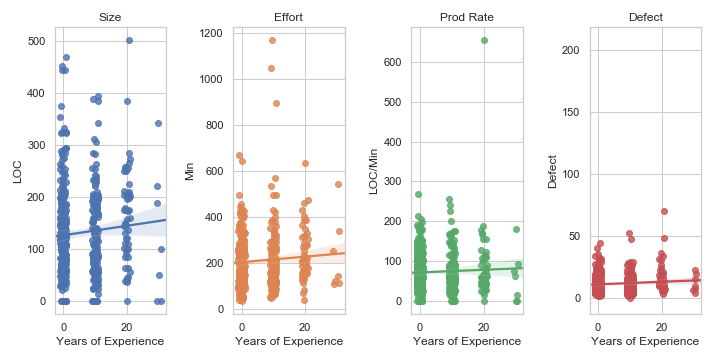
\includegraphics[width=\linewidth]{resources/h4_example_1.png}
\caption{H4 example plot}
\label{fig:h1e_example}
\end{center}
\end{figure}





% old table with stats without data
% \begin{table*}
% \centering
% \caption{H4: Years of experience has a negative influence on productivity. 
% A: with stats background, B: without stats background}
% \label{tab: h4}
% \begin{tabular}{|c|c|c|c|c|c|c|c|c|c|c|c|}
% \hline
% \textbf{Task} & \textbf{Experience} & \textbf{\begin{tabular}[c]{@{}c@{}}A \\ count\end{tabular}} & \textbf{\begin{tabular}[c]{@{}c@{}}B \\ count\end{tabular}} & \textbf{\begin{tabular}[c]{@{}c@{}}A\\ size\end{tabular}} & \textbf{\begin{tabular}[c]{@{}c@{}}B\\ size\end{tabular}} & \textbf{\begin{tabular}[c]{@{}c@{}}A\\ effort\end{tabular}} & \textbf{\begin{tabular}[c]{@{}c@{}}B\\ effort\end{tabular}} & \textbf{\begin{tabular}[c]{@{}c@{}}A\\ prod\_rate\end{tabular}} & \textbf{\begin{tabular}[c]{@{}c@{}}B\\ prod\_rate\end{tabular}} & \textbf{\begin{tabular}[c]{@{}c@{}}A\\ defect\end{tabular}} & \textbf{\begin{tabular}[c]{@{}c@{}}B\\ defect\end{tabular}} \\ \hline
%  & \textbf{0} & 428 & 489 & \cellcolor[HTML]{C0C0C0}83 & 88 & \cellcolor[HTML]{C0C0C0}169 & 135 & \cellcolor[HTML]{C0C0C0}52 & 63 & \cellcolor[HTML]{C0C0C0}8 & 6 \\ \cline{2-12} 
%  & \textbf{1-10} & 299 & 199 & \cellcolor[HTML]{C0C0C0}72 & \cellcolor[HTML]{C0C0C0}44 & \cellcolor[HTML]{C0C0C0}132 & \cellcolor[HTML]{C0C0C0}97 & \cellcolor[HTML]{C0C0C0}53 & 52 & \cellcolor[HTML]{C0C0C0}7 & \cellcolor[HTML]{C0C0C0}5 \\ \cline{2-12} 
%  & \textbf{11-20} & 124 & 39 & 107 & 106 & 201 & 212 & \cellcolor[HTML]{C0C0C0}52 & 61 & 10 & 9 \\ \cline{2-12} 
% \multirow{-4}{*}{\textbf{1}} & \textbf{20+} & 23 & 18 & 114 & \cellcolor[HTML]{C0C0C0}60 & 233 & 207 & \cellcolor[HTML]{C0C0C0}61 & \cellcolor[HTML]{C0C0C0}27 & 12 & 7 \\ \hline
%  & \textbf{0} & 428 & 489 & \cellcolor[HTML]{C0C0C0}63 & 62 & \cellcolor[HTML]{C0C0C0}156 & 138 & \cellcolor[HTML]{C0C0C0}40 & \cellcolor[HTML]{C0C0C0}46 & \cellcolor[HTML]{C0C0C0}5 & \cellcolor[HTML]{C0C0C0}5 \\ \cline{2-12} 
%  & \textbf{1-10} & 299 & 199 & \cellcolor[HTML]{C0C0C0}58 & \cellcolor[HTML]{C0C0C0}53 & \cellcolor[HTML]{C0C0C0}148 & \cellcolor[HTML]{C0C0C0}123 & \cellcolor[HTML]{C0C0C0}42 & \cellcolor[HTML]{C0C0C0}43 & \cellcolor[HTML]{C0C0C0}6 & \cellcolor[HTML]{C0C0C0}5 \\ \cline{2-12} 
%  & \textbf{11-20} & 124 & 39 & \cellcolor[HTML]{C0C0C0}69 & 65 & 188 & 138 & \cellcolor[HTML]{C0C0C0}41 & \cellcolor[HTML]{C0C0C0}48 & \cellcolor[HTML]{C0C0C0}7 & \cellcolor[HTML]{C0C0C0}5 \\ \cline{2-12} 
% \multirow{-4}{*}{\textbf{2}} & \textbf{20+} & 23 & 18 & \cellcolor[HTML]{C0C0C0}79 & 69 & \cellcolor[HTML]{C0C0C0}162 & 174 & \cellcolor[HTML]{C0C0C0}48 & \cellcolor[HTML]{C0C0C0}39 & \cellcolor[HTML]{C0C0C0}6 & \cellcolor[HTML]{C0C0C0}3 \\ \hline
%  & \textbf{0} & 428 & 489 & \cellcolor[HTML]{C0C0C0}73 & \cellcolor[HTML]{C0C0C0}75 & \cellcolor[HTML]{C0C0C0}191 & \cellcolor[HTML]{C0C0C0}179 & \cellcolor[HTML]{C0C0C0}40 & 42 & \cellcolor[HTML]{C0C0C0}6 & \cellcolor[HTML]{C0C0C0}6 \\ \cline{2-12} 
%  & \textbf{1-10} & 299 & 199 & \cellcolor[HTML]{C0C0C0}73 & \cellcolor[HTML]{C0C0C0}57 & \cellcolor[HTML]{C0C0C0}182 & \cellcolor[HTML]{C0C0C0}160 & \cellcolor[HTML]{C0C0C0}43 & \cellcolor[HTML]{C0C0C0}37 & \cellcolor[HTML]{C0C0C0}6 & \cellcolor[HTML]{C0C0C0}5 \\ \cline{2-12} 
%  & \textbf{11-20} & 124 & 39 & \cellcolor[HTML]{C0C0C0}89 & \cellcolor[HTML]{C0C0C0}98 & \cellcolor[HTML]{C0C0C0}225 & 228 & \cellcolor[HTML]{C0C0C0}42 & 44 & 7 & \cellcolor[HTML]{C0C0C0}8 \\ \cline{2-12} 
% \multirow{-4}{*}{\textbf{3}} & \textbf{20+} & 23 & 18 & \cellcolor[HTML]{C0C0C0}84 & \cellcolor[HTML]{C0C0C0}75 & \cellcolor[HTML]{C0C0C0}249 & 239 & \cellcolor[HTML]{C0C0C0}49 & \cellcolor[HTML]{C0C0C0}36 & 12 & \cellcolor[HTML]{C0C0C0}6 \\ \hline
%  & \textbf{0} & 428 & 489 & \cellcolor[HTML]{C0C0C0}72 & 74 & \cellcolor[HTML]{C0C0C0}161 & \cellcolor[HTML]{C0C0C0}141 & \cellcolor[HTML]{C0C0C0}43 & 52 & \cellcolor[HTML]{C0C0C0}4 & \cellcolor[HTML]{C0C0C0}4 \\ \cline{2-12} 
%  & \textbf{1-10} & 299 & 199 & \cellcolor[HTML]{C0C0C0}71 & \cellcolor[HTML]{C0C0C0}60 & \cellcolor[HTML]{C0C0C0}155 & \cellcolor[HTML]{C0C0C0}123 & \cellcolor[HTML]{C0C0C0}48 & 51 & \cellcolor[HTML]{C0C0C0}4 & \cellcolor[HTML]{C0C0C0}4 \\ \cline{2-12} 
%  & \textbf{11-20} & 124 & 39 & 87 & 90 & 190 & 203 & \cellcolor[HTML]{C0C0C0}46 & 48 & 6 & \cellcolor[HTML]{C0C0C0}4 \\ \cline{2-12} 
% \multirow{-4}{*}{\textbf{4}} & \textbf{20+} & 23 & 18 & 83 & 87 & 236 & 229 & \cellcolor[HTML]{C0C0C0}36 & \cellcolor[HTML]{C0C0C0}32 & 7 & \cellcolor[HTML]{C0C0C0}5 \\ \hline
%  & \textbf{0} & 428 & 489 & \cellcolor[HTML]{C0C0C0}81 & 83 & \cellcolor[HTML]{C0C0C0}178 & 161 & \cellcolor[HTML]{C0C0C0}44 & 52 & \cellcolor[HTML]{C0C0C0}5 & \cellcolor[HTML]{C0C0C0}5 \\ \cline{2-12} 
%  & \textbf{1-10} & 299 & 199 & \cellcolor[HTML]{C0C0C0}77 & \cellcolor[HTML]{C0C0C0}71 & \cellcolor[HTML]{C0C0C0}166 & \cellcolor[HTML]{C0C0C0}135 & \cellcolor[HTML]{C0C0C0}47 & 52 & \cellcolor[HTML]{C0C0C0}5 & \cellcolor[HTML]{C0C0C0}4 \\ \cline{2-12} 
%  & \textbf{11-20} & 124 & 39 & \cellcolor[HTML]{C0C0C0}89 & 90 & \cellcolor[HTML]{C0C0C0}201 & 238 & \cellcolor[HTML]{C0C0C0}46 & \cellcolor[HTML]{C0C0C0}43 & 7 & 6 \\ \cline{2-12} 
% \multirow{-4}{*}{\textbf{5}} & \textbf{20+} & 23 & 18 & \cellcolor[HTML]{C0C0C0}95 & 88 & \cellcolor[HTML]{C0C0C0}219 & 248 & \cellcolor[HTML]{C0C0C0}38 & \cellcolor[HTML]{C0C0C0}38 & 9 & \cellcolor[HTML]{C0C0C0}5 \\ \hline
%  & \textbf{0} & 428 & 489 & \cellcolor[HTML]{C0C0C0}151 & \cellcolor[HTML]{C0C0C0}152 & \cellcolor[HTML]{C0C0C0}322 & 259 & \cellcolor[HTML]{C0C0C0}47 & 56 & \cellcolor[HTML]{C0C0C0}8 & \cellcolor[HTML]{C0C0C0}6 \\ \cline{2-12} 
%  & \textbf{1-10} & 299 & 199 & \cellcolor[HTML]{C0C0C0}148 & \cellcolor[HTML]{C0C0C0}133 & \cellcolor[HTML]{C0C0C0}281 & \cellcolor[HTML]{C0C0C0}210 & \cellcolor[HTML]{C0C0C0}51 & 57 & \cellcolor[HTML]{C0C0C0}7 & \cellcolor[HTML]{C0C0C0}6 \\ \cline{2-12} 
%  & \textbf{11-20} & 124 & 39 & 175 & 203 & 373 & 416 & \cellcolor[HTML]{C0C0C0}48 & \cellcolor[HTML]{C0C0C0}46 & 11 & 11 \\ \cline{2-12} 
% \multirow{-4}{*}{\textbf{6}} & \textbf{20+} & 23 & 18 & 182 & 176 & 455 & 548 & \cellcolor[HTML]{C0C0C0}42 & \cellcolor[HTML]{C0C0C0}30 & 14 & 9 \\ \hline
%  & \textbf{0} & 428 & 489 & \cellcolor[HTML]{C0C0C0}77 & \cellcolor[HTML]{C0C0C0}82 & 215 & \cellcolor[HTML]{C0C0C0}198 & 37 & 43 & \cellcolor[HTML]{C0C0C0}5 & \cellcolor[HTML]{C0C0C0}5 \\ \cline{2-12} 
%  & \textbf{1-10} & 299 & 199 & \cellcolor[HTML]{C0C0C0}80 & \cellcolor[HTML]{C0C0C0}77 & \cellcolor[HTML]{C0C0C0}194 & \cellcolor[HTML]{C0C0C0}165 & 41 & 42 & \cellcolor[HTML]{C0C0C0}4 & \cellcolor[HTML]{C0C0C0}4 \\ \cline{2-12} 
%  & \textbf{11-20} & 124 & 39 & \cellcolor[HTML]{C0C0C0}87 & \cellcolor[HTML]{C0C0C0}106 & 229 & 267 & 37 & 42 & 6 & 6 \\ \cline{2-12} 
% \multirow{-4}{*}{\textbf{7}} & \textbf{20+} & 23 & 18 & \cellcolor[HTML]{C0C0C0}80 & \cellcolor[HTML]{C0C0C0}79 & 280 & 367 & \cellcolor[HTML]{C0C0C0}32 & \cellcolor[HTML]{C0C0C0}21 & 8 & 9 \\ \hline
%  & \textbf{0} & 428 & 489 & \cellcolor[HTML]{C0C0C0}76 & 78 & 178 & 151 & \cellcolor[HTML]{C0C0C0}41 & \cellcolor[HTML]{C0C0C0}47 & \cellcolor[HTML]{C0C0C0}4 & \cellcolor[HTML]{C0C0C0}3 \\ \cline{2-12} 
%  & \textbf{1-10} & 299 & 199 & \cellcolor[HTML]{C0C0C0}76 & \cellcolor[HTML]{C0C0C0}48 & \cellcolor[HTML]{C0C0C0}163 & \cellcolor[HTML]{C0C0C0}100 & \cellcolor[HTML]{C0C0C0}46 & \cellcolor[HTML]{C0C0C0}47 & \cellcolor[HTML]{C0C0C0}4 & \cellcolor[HTML]{C0C0C0}3 \\ \cline{2-12} 
%  & \textbf{11-20} & 124 & 39 & \cellcolor[HTML]{C0C0C0}97 & 100 & 215 & 262 & \cellcolor[HTML]{C0C0C0}42 & \cellcolor[HTML]{C0C0C0}40 & 6 & 7 \\ \cline{2-12} 
% \multirow{-4}{*}{\textbf{8}} & \textbf{20+} & 23 & 18 & 87 & 96 & 253 & 223 & \cellcolor[HTML]{C0C0C0}36 & \cellcolor[HTML]{C0C0C0}27 & 7 & 4 \\ \hline
%  & \textbf{0} & 428 & 489 & \cellcolor[HTML]{C0C0C0}134 & 149 & \cellcolor[HTML]{C0C0C0}296 & 265 & \cellcolor[HTML]{C0C0C0}46 & 53 & \cellcolor[HTML]{C0C0C0}7 & \cellcolor[HTML]{C0C0C0}6 \\ \cline{2-12} 
%  & \textbf{1-10} & 299 & 199 & \cellcolor[HTML]{C0C0C0}141 & \cellcolor[HTML]{C0C0C0}131 & \cellcolor[HTML]{C0C0C0}282 & \cellcolor[HTML]{C0C0C0}219 & \cellcolor[HTML]{C0C0C0}53 & 54 & \cellcolor[HTML]{C0C0C0}6 & \cellcolor[HTML]{C0C0C0}5 \\ \cline{2-12} 
%  & \textbf{11-20} & 124 & 39 & \cellcolor[HTML]{C0C0C0}167 & 172 & 359 & 390 & \cellcolor[HTML]{C0C0C0}46 & 42 & 11 & 9 \\ \cline{2-12} 
% \multirow{-4}{*}{\textbf{9}} & \textbf{20+} & 23 & 18 & \cellcolor[HTML]{C0C0C0}149 & 145 & 352 & 466 & \cellcolor[HTML]{C0C0C0}38 & \cellcolor[HTML]{C0C0C0}29 & 13 & 7 \\ \hline
%  & \textbf{0} & 428 & 489 & \cellcolor[HTML]{C0C0C0}211 & 202 & \cellcolor[HTML]{C0C0C0}359 & 304 & \cellcolor[HTML]{C0C0C0}54 & 64 & \cellcolor[HTML]{C0C0C0}7 & \cellcolor[HTML]{C0C0C0}6 \\ \cline{2-12} 
%  & \textbf{1-10} & 299 & 199 & \cellcolor[HTML]{C0C0C0}217 & \cellcolor[HTML]{C0C0C0}182 & \cellcolor[HTML]{C0C0C0}334 & \cellcolor[HTML]{C0C0C0}255 & \cellcolor[HTML]{C0C0C0}61 & 64 & \cellcolor[HTML]{C0C0C0}7 & \cellcolor[HTML]{C0C0C0}5 \\ \cline{2-12} 
%  & \textbf{11-20} & 124 & 39 & \cellcolor[HTML]{C0C0C0}232 & 239 & 453 & 469 & \cellcolor[HTML]{C0C0C0}54 & \cellcolor[HTML]{C0C0C0}54 & 10 & 11 \\ \cline{2-12} 
% \multirow{-4}{*}{\textbf{10}} & \textbf{20+} & 23 & 18 & \cellcolor[HTML]{C0C0C0}229 & 249 & 479 & 601 & \cellcolor[HTML]{C0C0C0}47 & \cellcolor[HTML]{C0C0C0}37 & 15 & 9 \\ \hline
% \multicolumn{4}{|c|}{\textit{\textbf{TOP RANKED}}} & \textit{\textbf{\begin{tabular}[c]{@{}c@{}}0=10, \\ 1-10=10,\\ 11-20=7,\\ 20+=4\end{tabular}}} & \textit{\textbf{\begin{tabular}[c]{@{}c@{}}0=3, \\ 1-10=10,\\ 11-20=2,\\ 20+=3\end{tabular}}} & \textit{\textbf{\begin{tabular}[c]{@{}c@{}}0=8, \\ 1-10=10,\\ 11-20=2,\\ 20+=3\end{tabular}}} & \textit{\textbf{\begin{tabular}[c]{@{}c@{}}0=3, \\ 1-10=10,\\ 11-20=0,\\ 20+=0\end{tabular}}} & \textit{\textbf{\begin{tabular}[c]{@{}c@{}}0=9, \\ 1-10=9,\\ 11-20=9,\\ 20+=10\end{tabular}}} & \textit{\textbf{\begin{tabular}[c]{@{}c@{}}0=10,\\ 1-10=9,\\ 11-20=6,\\ 20+=2\end{tabular}}} & \textit{\textbf{\begin{tabular}[c]{@{}c@{}}0=10,\\ 1-10=10,\\ 11-20=1,\\ 30+=1\end{tabular}}} & \textit{\textbf{\begin{tabular}[c]{@{}c@{}}0=9,\\ 1-10=10,\\ 11-20=3,\\ 20+=4\end{tabular}}} \\ \hline
% \end{tabular}
% \end{table*}









\section{Appendices}

If your work needs an appendix, add it before the
``\verb|\end{document}|'' command at the conclusion of your source
document.

Start the appendix with the ``\verb|appendix|'' command:
\begin{verbatim}
  \appendix
\end{verbatim}
and note that in the appendix, sections are lettered, not
numbered. This document has two appendices, demonstrating the section
and subsection identification method.

\section{SIGCHI Extended Abstracts}

The ``\verb|sigchi-a|'' template style (available only in \LaTeX\ and
not in Word) produces a landscape-orientation formatted article, with
a wide left margin. Three environments are available for use with the
``\verb|sigchi-a|'' template style, and produce formatted output in
the margin:
\begin{itemize}
\item {\verb|sidebar|}:  Place formatted text in the margin.
\item {\verb|marginfigure|}: Place a figure in the margin.
\item {\verb|margintable|}: Place a table in the margin.
\end{itemize}

%%
%% The acknowledgments section is defined using the "acks" environment
%% (and NOT an unnumbered section). This ensures the proper
%% identification of the section in the article metadata, and the
%% consistent spelling of the heading.
\begin{acks}
To Robert, for the bagels and explaining CMYK and color spaces.
\end{acks}

%%
%% The next two lines define the bibliography style to be used, and
%% the bibliography file.
\bibliographystyle{ACM-Reference-Format}
\bibliography{ref}

%%
%% If your work has an appendix, this is the place to put it.
\appendix


\end{document}
\endinput
%%
%% End of file `sample-authordraft.tex'.
